\documentclass{article}
\usepackage[margin=1.5cm,bottom=2cm]{geometry}
\usepackage{fancyhdr}
\usepackage{graphicx}
\usepackage{amsmath}
\usepackage{enumitem}
\pagestyle{fancy}

\begin{document}
\fancyhead[L]{ 
\includegraphics[width=2cm]{au_logo.png} }
\fancyhead[R]{PHYS 4220: Computational Physics}
\fancyfoot[C]{\thepage}
\vspace*{0cm}
\begin{center}
	{\LARGE \textbf{Homework 2}}\\
	\vspace{0.25cm}
	{\Large Due: Friday, September 18}
\end{center}

\newcommand{\textbook}{\textit{Giordano}}
{\large \textbf{Terminal Velocity} }
\begin{enumerate}
	\item An over-eager skydiver has jumped out of the plane without their parachute! We want to estimate the conditions under which a second skydiver can reach the first skydiver. The forces acting on the skydivers are: $F_\mathrm{grav}=mg$, $F_\mathrm{drag}=\frac{1}{2}C\rho A v^2$. Assume $C=1$. We will work in SI units in this problem. Assume that the plane is flying at an altitude of $5,000$ meters and neglect any initial velocity of the skydivers. The air density $\rho$ is approximately 1.225 kg/m$^3$. Each skydiver has a mass of 70 kg. The first skydiver lays flat as they fall, with a cross-sectional area of $A=1$ m$^2$. 
	\begin{enumerate}
		\item 	If the second skydiver leaves the plane 30 s after the first, what cross-sectional area must they attain in order to catch the first skydiver in time to deploy a parachute ($y=500$ meters?)
		\item In reality, the air density $\rho$ is not constant with altitude, but changes as $\rho(y) = \rho_0 e^{-\frac{y}{y_0}}$, where $\rho_0=$1.225 kg/m$^3$ is the density at sea level, and $y_0=10^4$ meters is the scale height of the atmosphere. How does this change your answer?
	\end{enumerate}


\end{enumerate}

{\large \textbf{Escape Velocity} }
\begin{enumerate}[resume]
	\item Consider a projectile launched from the surface of the Earth. Assume the projectile is able to travel far enough from the center of the Earth that gravitational acceleration is no longer constant ($F\mathrm{grav}\approx mg$ does \textit{not} hold.) You may, however, neglect air resistance for this problem.
	\begin{enumerate}
		\item Write and normalize the equation of motion (the differential equation) for the projectile. \textit{Hint: the radius of the earth $R_E$ makes a good choice for length units, then let $\frac{v_0}{t_0}=g=\frac{G M_E}{R_E^2}$.} You should arrive at an equation which is independent of mass or any fundamental constants.
		\item Solve this system numerically. There exists a specific velocity, $v_\infty$, beyond which the projectile will never return to Earth. Approximate this value using your numerical solution. \textit{Hint: If you choose not to obtain this result analytically, the best way is just to try different values of $v_i$ and plot the corresponding motion. In the units described above, $v_\infty$ will be $\sim 1$ (it will be a number of order one, not $10^{-6} or 10,000$). This should help narrow your search. }
		\item \textbf{Bonus:} While your equation of motion from (a) is difficult to solve analytically, we can consider the initial and final energy of the projectile to derive $v_\infty$. The projectile will escape if, and only if, its initial kinetic energy is sufficient to overcome the work done by the gravitational force from $r=R_E$ to $r=\infty$. Use this information to derive $v_\infty$, assuming the projectile's motion is non-relativistic.
	\end{enumerate}
\end{enumerate}

{\large \textbf{RLC Circuit} }
\begin{figure}[!ht]
	\centering
	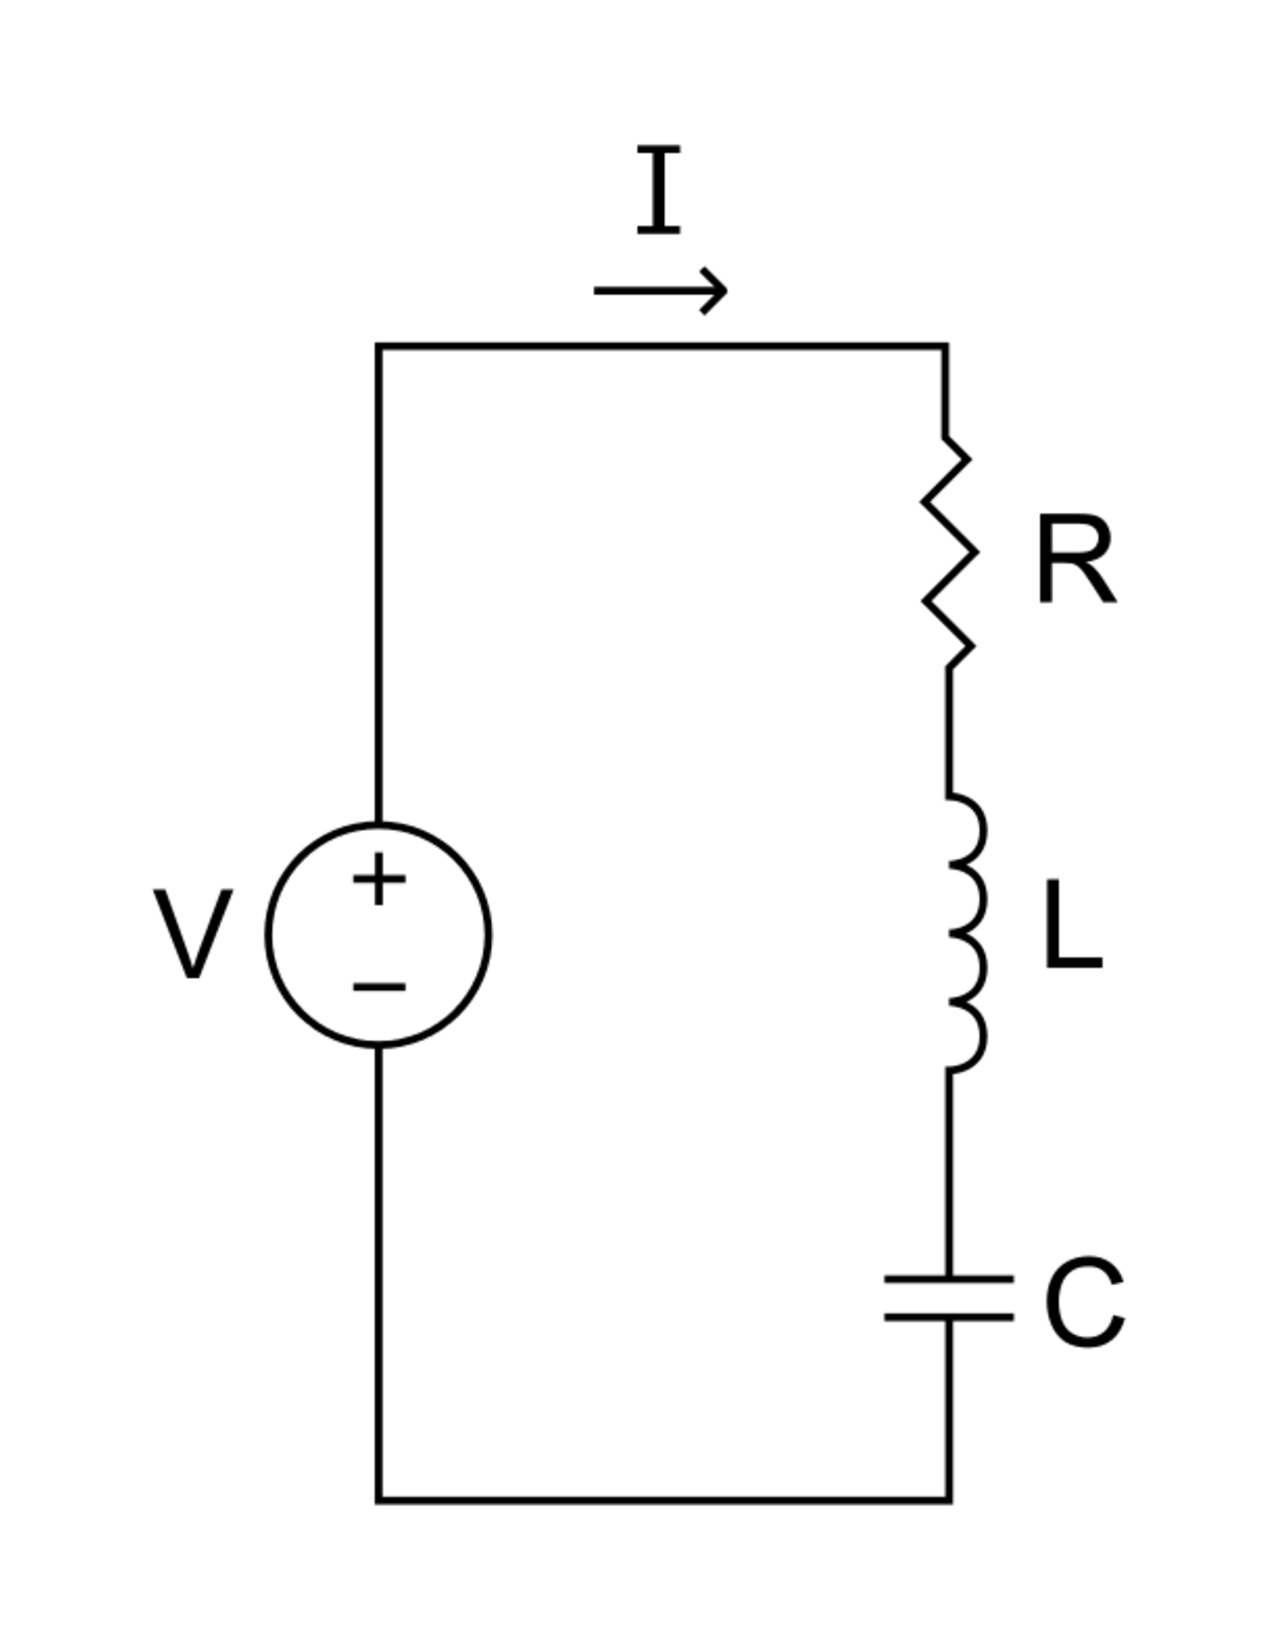
\includegraphics[width=5cm]{RLC_series_circuit_v1.pdf}
\end{figure}
\begin{enumerate}[resume]
	\item Consider the above circuit. We can use Kirchhoff's loop rule to obtain the following differential equation for the current in the circuit as a function of time:
	\begin{equation*}
		\frac{d^2I}{dt^2}+\frac{R}{L}\frac{dI}{dt} + \frac{1}{LC}I = 0
	\end{equation*}
	Where $R$ is the resistance of the resistor and has dimensions [$R$]=$ML^2/I^2T^3$, $L$ is the inductance of the inductor with dimensions [$L$]=$ML^2/T^2I^2$, and $C$ is the capacitance with dimensions: [$C$]=$T^4I^2/ML^2$. $R/L$ therefore has dimensions of $1/T$, $LC$ has dimensions of $T$, $RC$ has dimensions of $T$. Assume $I(0)=I_0$, $\frac{dI}{dt}(0)=0$.
	\begin{enumerate}
		\item Using $\Omega_0=\frac{1}{t_0}=\frac{1}{\sqrt{LC}}$ as your time unit, normalize the differential equation. Show that your resulting equation depends solely on the dimensionless ``damping factor'' $Q^2=\frac{RC}{L/R}$, which is the ratio of time constants for an $RC$ circuit and an $RL$ circuit.
		\item This equation is identical to our linear, damped pendulum. What are the conditions for underdamped, overdamped, and critically damped behavior? Solve numerically and plot and example of each.
		\item \textbf{Bonus:} Obtain an analytical solution to the above equation.
	\end{enumerate}
	
\end{enumerate}
\end{document}